\chapter{Introduction}
\openepigraph{Nanos gigantum humeris insidentes.}{Bernard of Chartres}
\openepigraph{If I have seen further, it is by standing on the shoulders of giants.}{Isaac Newton}

Artificial Intelligence has transformed our industry in the recent past. With every iteration of every conference we hear a buzz around smaller and faster deployments of neural networks, along with a constant push in making the hardware that supports this boom more efficient. From companies investing millions in specialized accelerators (ASICs) for their specific application to hardware companies transforming their business strategy to keep up with the buzz, more (inference) for less (energy and time) seems to be the holy grail of the coming decade. 

\begin{figure}
    \centering
    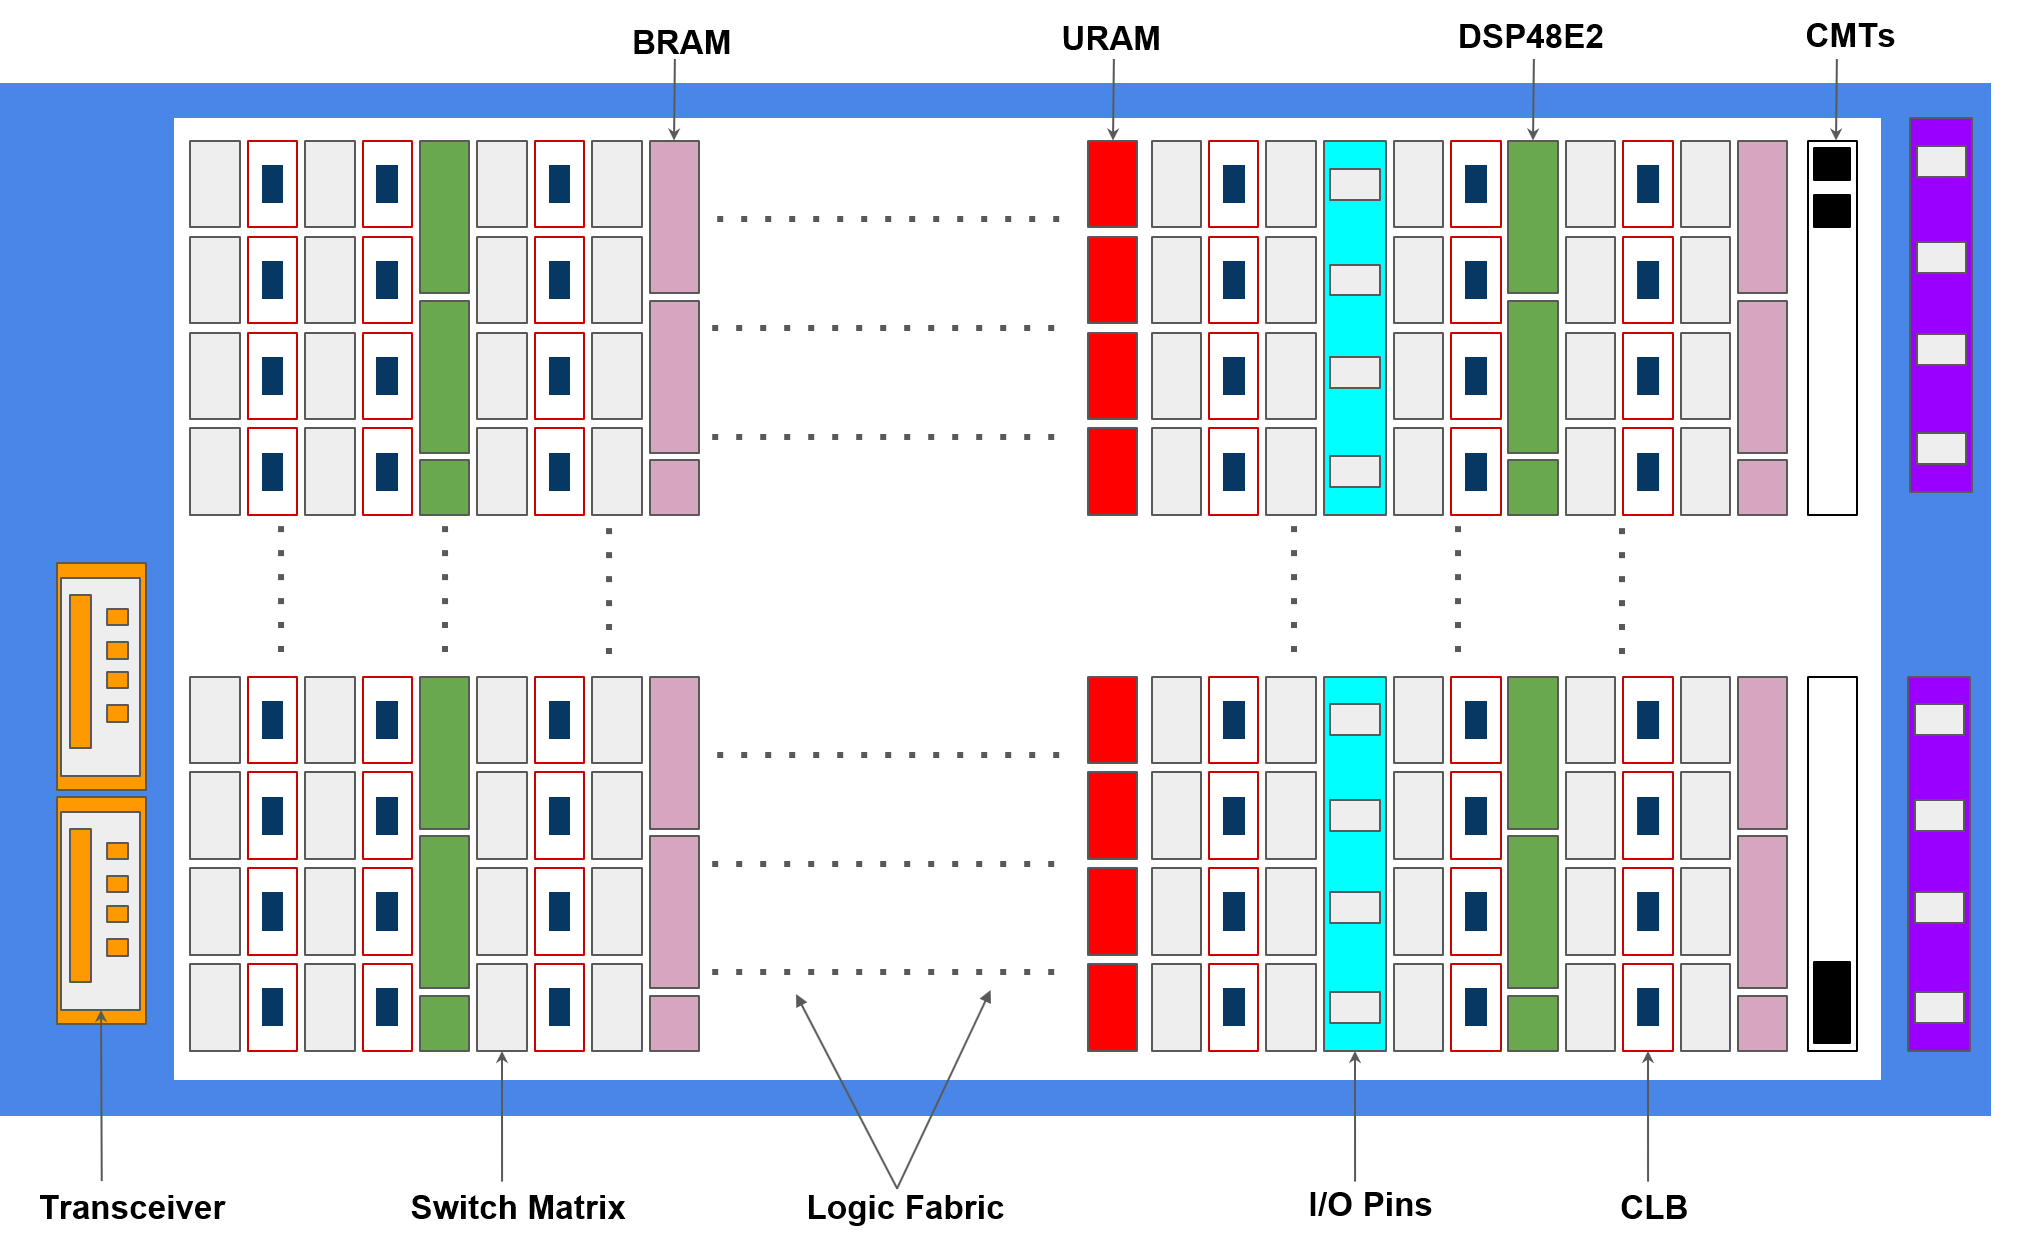
\includegraphics[width=400pt]{figures/bison/FPGA.png}
    \caption{Example UltraScale+ layout}
    \label{fig:fpga}
\end{figure}


This thesis hopes to focus on a novel method of representing neural networks, that lends us advantages during inference. We hope to identify appropriate use cases for this method of developing neural network topologies, and gain insight into the behavior of  aggressive sparsification and quantization of neural networks along with the ramifications of design decisions to hardware cost.


\section{Field-Programmable Gated Arrays}

\marginpar{\centering
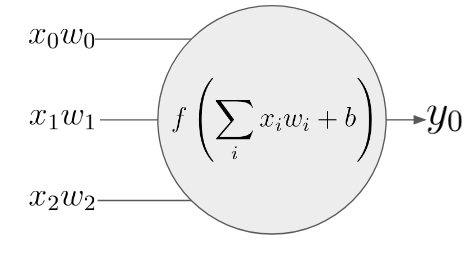
\includegraphics[width=120pt]{figures/bison/neuron.png}
\captionof{figure}{Illustration of a neuron.}
\label{fig:neuron}
% \endgroup
}



\marginpar{\centering
\vspace{10pt}
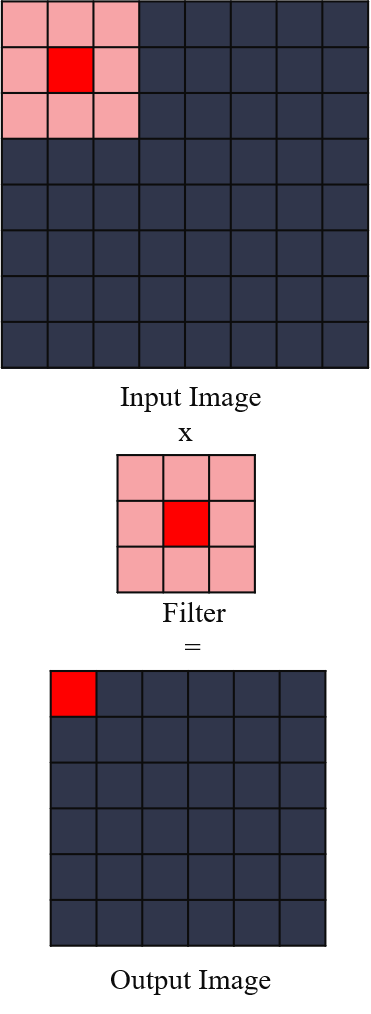
\includegraphics[width=100pt]{figures/bison/convolutionT.png}
\captionof{figure}{Illustrating Convolution.}
\label{fig:convolution}
% \endgroup
}

The basic architecture of a Xilinx FPGA is a two-dimensional array of digital logic elements, that are grouped into Configurable Logic Blocks (CLBs). Each CLB is composed of flip-flops, Look-Up Tables (LUTs). These CLBs are connected together with programmable interconnects and switch matrices. Modern FPGAs have many improvements, one of which is larger memory blocks Block RAMs (BRAMs) and Ultra RAMs (URAMs). These larger memory elements are dense and fast, and have many applications. Modern FPGAs also have integrated arithmetic blocks (DSPs) which are capable of multiplication, addition/subtraction, and other logical functions. \\
\cref{fig:fpga} illustrates the resource layout for an UltraScale+ FPGA. At a high level of abstraction, the FPGA device has vertical regions with an array of resources. A large proportion of the FPGA fabric is dedicated to general purpose logic. CLBs (Configurable Logic Blocks) that are composed of LUTs and Flip Flops. The I/O Blocks are arranged in banks and support a wide variety of interfacing standards. The DSP48E2s are Digital Signal Processing slices that support arithmetic, as well as can be used for barrel shifting, pattern detection, and much more.\\
From \cref{st:tab:fpgaresources}, it becomes evident that we have far more LUTs than we have DSP slices. While a DSP slice $(DSP48E2)$ has functionality ranging from a 48-bit logic unit to being a $27\times18$ two's complement multiplier, our approach hopes to sparsify and quantize neural networks to an extent where it becomes more beneficial to configure these LUTs to map to neurons. \\
One of FPGA's fundamental building block is a '$K-LUT$', which can perform any $K$ input boolean operation. In this thesis, we study how niche domains can benefit vastly by viewing a neuron as an boolean function transform, which maps $X$ input bits to $Y$ output bits. This is particularly intriguing as we can convert a neuron to a configuration of such '$K-LUTs$' and achieve high throughput. \\ 

We propose utilizing the individual $K-LUTs$ to perform arbitrary non-linear functions to a fixed number of activation bits. The advantage is that we can have full-precision weights, and the result is discovering a sparse topology with activation quantization. 



\begin{table}
    \begin{sidecaption}[FPGA Resource Table]{%
        Resources available in Xilinx  UltraScale\texttrademark FPGAs. Device names with a 'K' prefix refer to the Kintex\textregistered  UltraScale\texttrademark  FPGAs, names with a 'XCV' prefix refer to the Virtex\textregistered  UltraScale\texttrademark  FPGAs.
    }[st:tab:fpgaresources]
    \centering
    \begin{threeparttable}
    \renewcommand{\arraystretch}{1.2}
    \begin{tabular}{lrrrr}
        \toprule 
                                                %  & \multicolumn{3}{c}{\cref{st:alg:no_ls}} \\  
        Device                                   & CLB LUTs & BRAMs (18Kb) & DSP Slices  \\
        \midrule
        KU025 \                                  &  145,440  &  720      &     1,152   \\
        KU060\                                   &  331,680  & 2,160     &     2,760   \\
        XCVU065\                                 &  358,080  & 2,520     &     600   \\ 
        KU115\                                   &  663,360  & 4,320     &     5,520   \\ 
        XCVU440     \                            &  2,532,960& 5,040     &     2,880 \\ 
        \bottomrule
    \end{tabular}
    \end{threeparttable}
    \end{sidecaption}
\end{table}



% \vspace{30pt}
% \begin{figure}[t]
%     \begin{sidecaption}[Illustrating Convolution]{%
%             This image has been reproduced from~\cite{Baskin_2018}
%     }[fig:convolution]
%     \centering
%     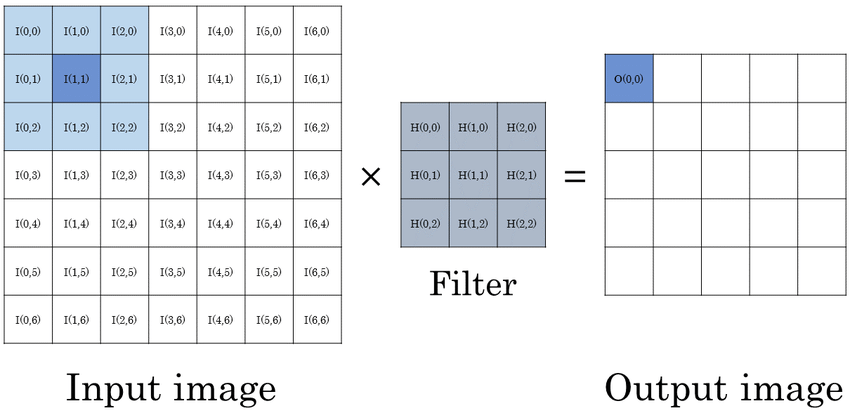
\includegraphics[width=250pt]{figures/bison/convolution.png}
%     \end{sidecaption}
% \end{figure}

\section{Deep Neural Networks}
A Deep Neural Network can be used for an array of tasks, from classification, segmentation, detection to actually generating new data after learning the semantics of the task. In our thesis, we focus on viewing each neuron as a boolean function, and limit ourselves to identification or classification tasks.

\newthoughtpar{Linear Layers}
We can think of a neuron in a linear layer as a function which applies a linear transformation on an input of dimension $I$ and results in an output of dimension $O$. We can further add a non-linearity to such a layer, like the ReLU activation function. In Figure \ref{fig:neuron}, we demonstrate a neuron of fan-in of 3, and has 1 output. From a boolean function perspective, if $x_{i}$ is the input, and $y_{0}$ is the output, and both the input and output are of 16-bit fixed point data-types, then we can expect the boolean function '$f$' to be $f : B^{48} \rightarrow B^{16}$, where $B = \{0, 1\}$. This would require a huge truth table, needing around $4.50\times10^{15}$ bits of storage. It is easy to see that such a neuron is unfeasible to implement on any FPGA. We therefore need to aggressively prune the number of inputs to such a neuron, as well as the bit-width of the input and outputs. Later in this document we will describe the relation of input and output bits of a neuron with the hardware cost as well, which will aid us in design decisions.

\newthoughtpar{Convolutional Layers}
Figure \ref{fig:convolution} represents a simple convolution operation, where the input image has 1 channel, and the filter depth is 1. It is natural to view these filters as neurons, that respond differently to different spatial features. When the filter correlates well with a region of the input image, the response in the corresponding output image is strong. Since the contents of the filter remain the same at inference, we can also represent a filter convolution with simple truth tables. Such a truth table would essentially represent the boolean function $f : B^{144} \rightarrow B^{16}$, where $B = \{0, 1\}$. This assumes that the Input and Output image pixels are all represented by 16-bit data-types. This is not a fair estimate of the dimensionality of the boolean function due to the fact that we are ignoring the number of input feature maps, which are considerably high in a typical convolutional neural network.


\subsection{Quantized Neural Networks}
Quantized Neural Networks have been a very attractive avenue for researchers in the deep learning community due to the benefits it provides for inference. Many techniques to quantize neural networks have been proposed, which broadly can be classified as deterministic and stochastic quantization. There are three components that are generally quantized. The weights, activations and the gradient. \\
We see notable inference time improvements in performance when quantizing weight and activations, while the primary benefit of quantizing gradients is to save on communication cost in distributed training. It is worth noting that it quantizing gradients is generally not advisable as high precision gradients are required to make the optimizer converge. \\
Ever since quantized neural networks have been explored, FPGA implementations of Neural Network accelerators have become increasingly better at inference with low precision bit-widths for both weights and activations. \cite{umuroglu+:FPGA2017finn} proposed BNN accelerators with a dataflow-style architecture where processing engines are instantiated for every layer. LUTs were heavily utilized to provide XNOR-Popcounts and accumulate operations and weights and intermediate activations were stored in BRAMs. This research also implemented a folding scheme to allow for larger networks to be mapped to smaller devices. \cite{wang2019lutnet} introduced LUTNet, that took a pruned version of ReBNet~\cite{ghasemzadeh2018rebnet} in which some of the XNOR-Popcount operations are mapped more effectively to $k$-input LUTs. \cite{murovivc2019massively} implemented binarized networks which have been fully unrolled and implemented directly into LUTs of a small FPGA. This unrolling allowed the synthesis optimization tool to simplify significant portions of the compute logic. \\

\subsection{Sparse Neural Networks}
In sparse neural networks, each layer of neurons receive input from only a few connections from the previous layer of activation. In typical dense layers, every neuron receives input from every activation from the previous layer. We identify three key methods to sparsify Deep Neural Networks; A Priori Fixed Sparsity, Iterative Pruning and Learned Sparsity. In A Priori Fixed Sparsity, a network is initialized with a certain connectivity pattern, which remains fixed throughout training. Two examples of this approach are Deep Expander Networks~\cite{prabhu2018deep} and RadiX-net~\cite{DBLP:journals/corr/abs-1905-00416}. Iterative pruning methods generally use the magnitude of weights to prune a dense network. Recent methods utilize other metrics for this task well. Learned Sparsity methods such as Discovering Neural Wirings~\cite{DBLP:journals/corr/abs-1906-00586} and Neuroevolution of Augmented Topologies~\cite{stanley2002evolving} are aproaches that use some form of learning to identify important connections, establishing and pruning connections as desired. 
% \section{Logic Synthesis}


% \begingroup\centering
% 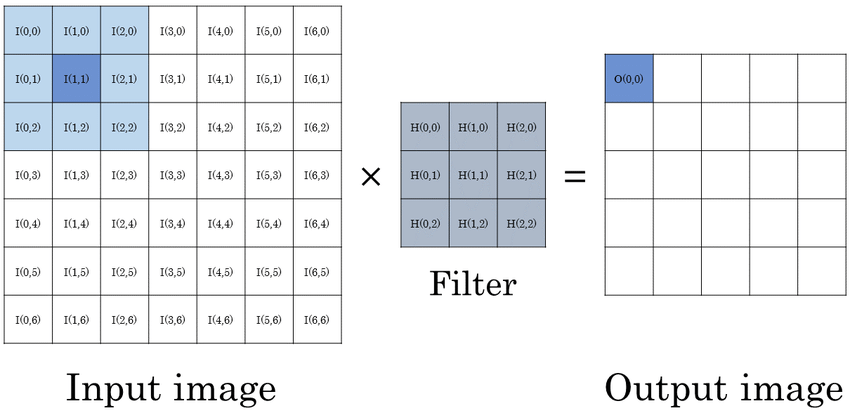
\includegraphics[width=250pt]{figures/bison/convolution.png}
% \captionof{figure}{Illustrating Convolution. This image has been reproduced from~\cite{Baskin_2018}}
% \label{fig:convolution}
% \endgroup

% /*
% Introduction
% The need for accelerators
%     CPUs, GPUs, ASICs, FPGAs.
% Background
%     FPGA and HW/SW Co-Design
%     Mapping Neurons to Hardware
%       Sparsity
%           Expander, Iterative, Momentum
%       Quantize
%           Activation brevitas
%           Non Linear
% LogicNet: A Library for Mapping HBBs to NEQs
%     Introduction
%     Components
%       Linear
%       Convolutions
%     Design Automation
%       TruthTableGen
%       VerilogGen
%       Synthesis
% Testing LogicNet
%     LogicNet4HEP
%       Introduction
%       Models
%     MNIST 
%       Models
% Concluding Remarks
%     Research Questions
%     Conclusion
% */